\section{Conclusion and Future Work}
We present a compact representation of PRT for \textbf{free form} deformable objects, informing of a non-linear model, namely a deep convolutional neural network, with significant memory savings demonstrated. We demonstrate that DeepPRT is able to produce good quality appearance estimations for deforming objects by only requiring the storage of the network parameters. In contrast, classic PRT methods require storing every single light-transport-state for each deformation pose, which in practice becomes unfeasible.

The model is able to extract the features of the dataset relevant to the light transfer function and thus generates good visual approximations for a wide spectrum of deformations, with resulting appearances that are practically indistinguishable from the ground truth.  

Moreover, our method shows much higher generalization properties than previous approaches, allowing deformations from much larger and less constrained deformation spaces.

%%%%%%%%%%%%%%%%%%%%%%%%%%%%% 
%\textit{\begin{figure*}
%  \centering
%    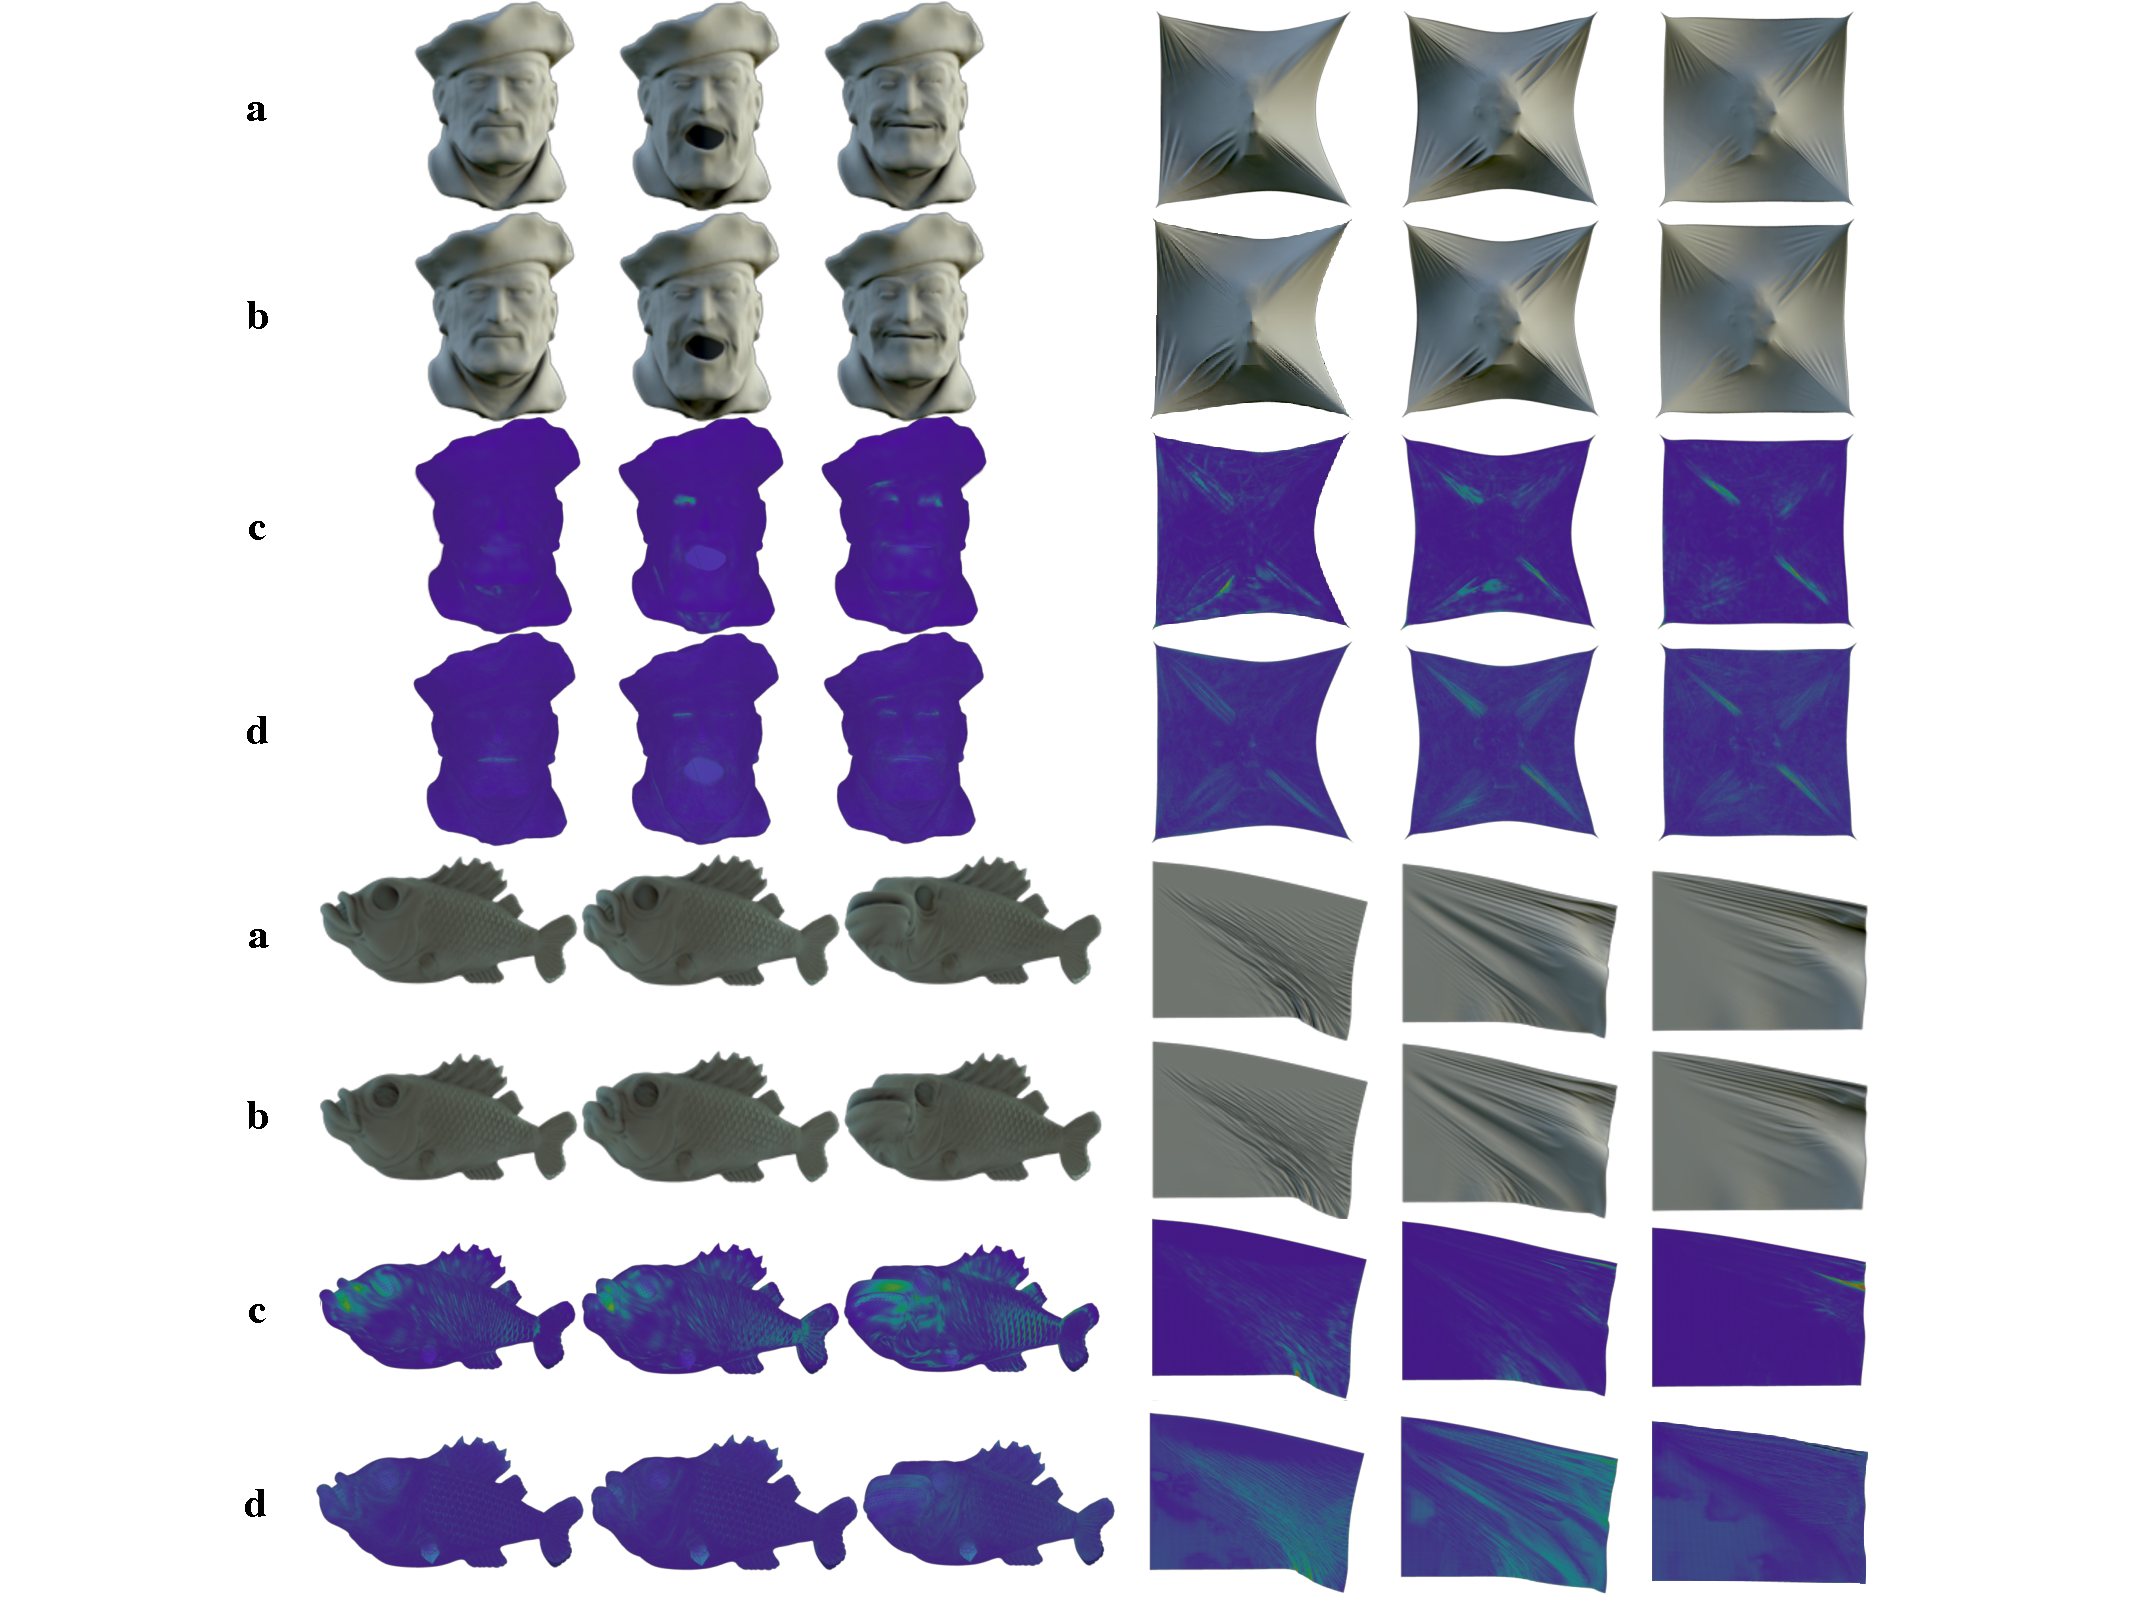
\includegraphics[width=0.5\paperwidth]{Figures/DPRT_quality_SSIM.pdf}
%     \caption{Prediction Quality:
%     a : ground truth appearance. b: predicted appearance. c: SSIM. d: L1-Error between ground truth and predicted transfer coefficients }
%     \label{Fig: DPRT_Quality}
%\end{figure*}}
\begin{figure}[H]
  \centering
    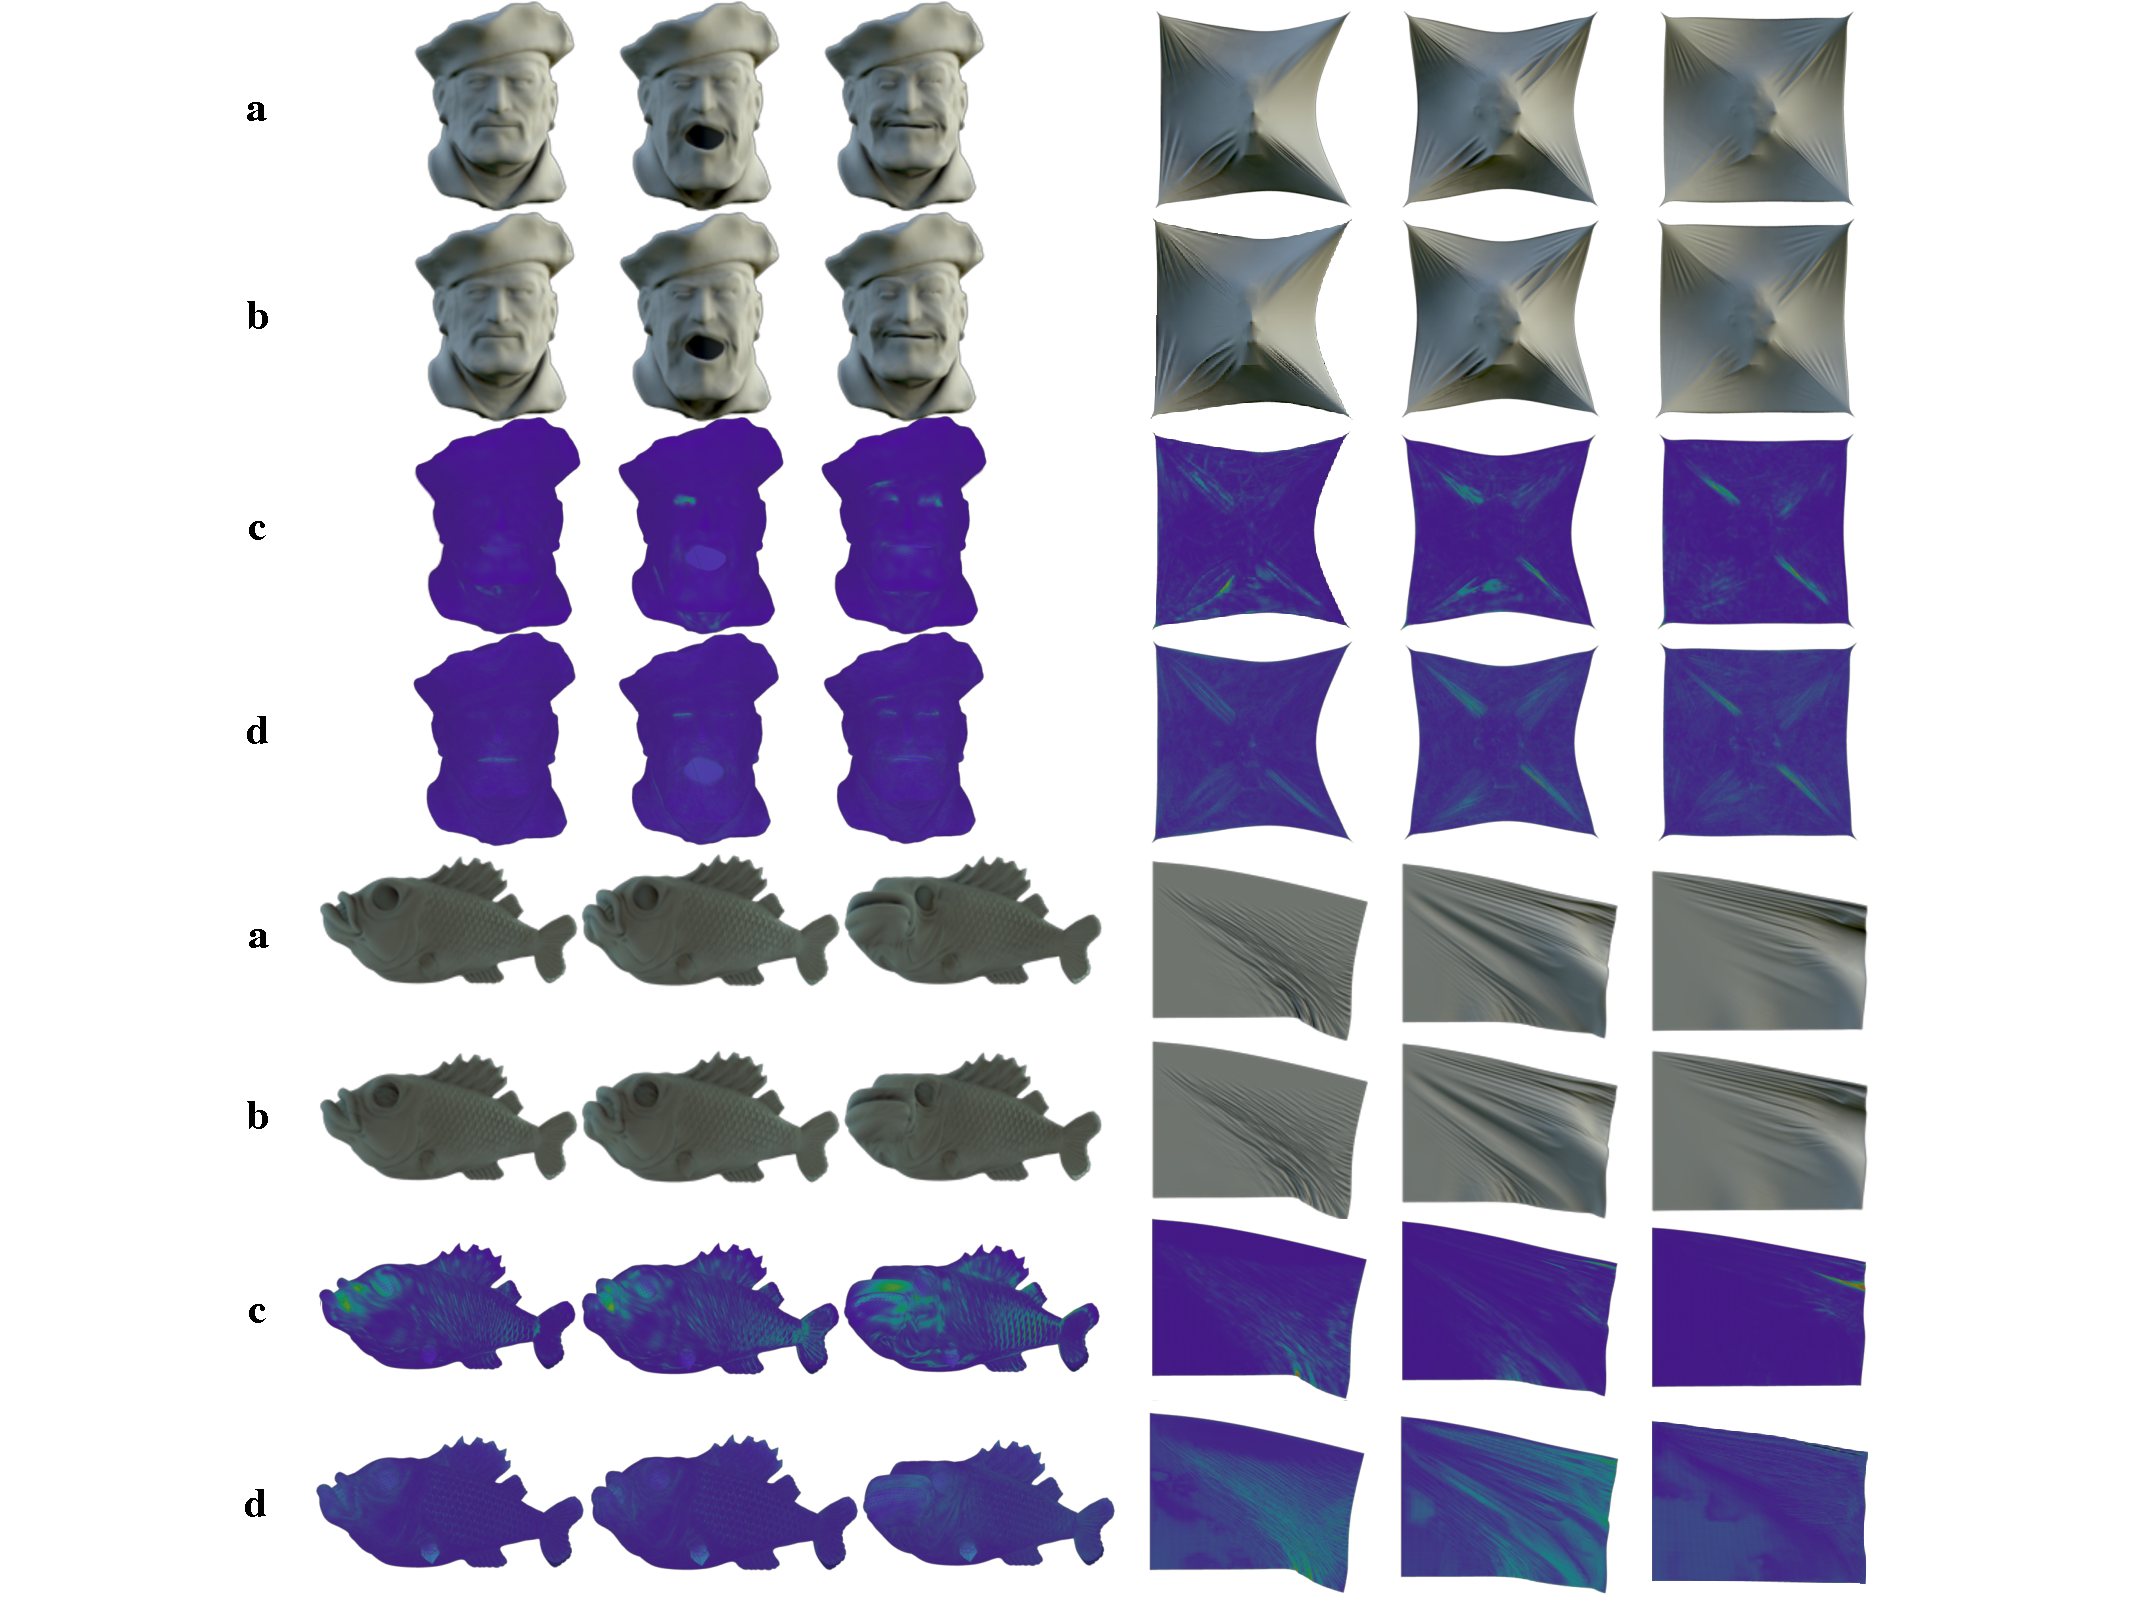
\includegraphics[width=1.0\textwidth]{Figures/DPRT_quality_SSIM.pdf}
     \caption{Prediction Quality:
     a) ground truth appearance. b) predicted appearance. c) SSIM. d) L1-Error between ground truth and predicted transfer coefficients }
     \label{Fig: DPRT_Quality}
\end{figure}

Although we showed DeepPRT can be much more compact than traditional PRT, our network is far from being fully optimized. Exploiting network compression and acceleration methods could be highly beneficial \cite{Survey_NN_Compression, Deep_Compression}. The memory requirements of a network can be reduced by using these network compression algorithms, without loosing accuracy, further reducing the storage requirements and speeding-up the inference time eventually enabling PRT to be applicable on deformable objects for real-time applications.

Moreover, other network topologies and/or cost functions could be explored in order to achieve better approximations, for instance, as proposed by Man et al. \shortcite{Deformable_UNet} to account for individual object deformations the use of deformable convolutions \cite{DeformableCNN} could be investigated. Further to the transfer function representation, a direct learning of more bespoke and compact representations \cite{Sloan2018} could also be applied in this context, such as sparse SH vectors or a CPCA-like compressed basis.

The particular choice of our basis functions (Spherical Harmonics), currently restricts our method to low-frequency lighting. However, an extension to all-frequencies is possible by fitting the model to an alternative representation of the transfer function $T$, such as non-linear Wavelets \cite{AllFrequencyPRT}.

The receptive field is a factor that can contribute to the performance of the CNN. Our network is adapted to the input image resolution with the intention to account for global feature extraction. Our particular network is deep enough to account for a receptive field that is almost the size of the input image of 256x256. By using other mappings (instead of the HM) such as the geometric-stretch parametrization, more flexible image resolutions can be used and possibly reduce the numbers of necessary layers. We assume and observe that geometry images, as experimented in this work, appropriately expose intrinsic properties of the surface deformations making the learning process more adept and due to the smoothness of the images more suitable for global feature extractions. However, a more explicit study follows regarding this assumption in evaluating performance of distant occluders and other distant or dislocated fully global illumination events.

The most significant further area of investigation for our method resides within the choice of our parametrization (harmonic map). In our tests, harmonic mapping performs well for modest curvature variations and is restricted to surfaces with one boundary (topological disks); however, using the geometric-stretch parametrization instead and further using the extension proposed by Praun and Hoppes \shortcite{Spherical_Parametrization}, the representation would be more accurate in the reconstruction of shape. The U-Net process in this context of sharp feature reconstruction and non-disk topologies would need additional measures. In particular, a treatment of the \textit{diffeomorphic} behavior \cite{detlefsen2018transformations} of these mappings appropriate to efficient deep learning of light transport for animating arbitrary surfaces would be interesting to further understand the representation trade-offs.


\begin{acks}
We would like to thank the anonymous reviewers for the insightful comments that greatly helped improve this manuscript. Also, Peter-Pike Sloan and Llogari Casas Cambra for corrections and assistance in the runtime rendered results preparation. This project has received funding from the European Union Horizon 2020 research and innovation program under the Marie Sklodowska-Curie grant agreement No. 642841.
\end{acks}